\documentclass{ximera}
\input{../preamble}

\addPrintStyle{..}

\begin{document}
	\author{Bart Lambregs, Vincent Gellens}
	\xmtitle{De positie}{}
    \xmsource\xmuitleg




% EERST: ALS JE IETS EEN PLAATS GEEFT IS DAT EEN PLAATSVECTOR 
% ALS IETS BEWEEGT BEWEEGT DEZE VECTOR 
% JE WILT EEN FUNCTIE DIE VOOR ELKE TIJD DE VECTOR GEEFT --> PLAATSFUNCTIE 



\subsection*{Positie en plaatsfunctie}

Met een referentiestelsel kan elke plaats van een puntmassa in de ruimte worden vastgelegd met een \textbf{positie- of plaatsvector}, algemeen genoteerd door \(\vec{r}\).
Afhankelijk van het aantal dimensies waarin de beweging beschreven wordt heeft deze plaatsvector één, twee of drie componenten volgens de gekozen assen, doorgaans \(\vec{x}\), \(\vec{y}\) en \(\vec{z}\) genaamd.
De (scalaire) getalcomponenten van deze vectoren zijn de plaatscoördinaten \(x\),\(y\) en \(z\).


\begin{image}
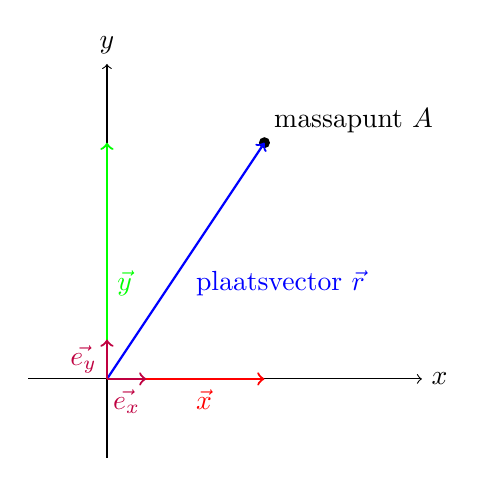
\begin{tikzpicture}
	\draw[->] (-1,0) -- (4,0) node[right] {$x$};
	\draw[->] (0,-1) -- (0,4) node[above] {$y$};
  
	\coordinate (A) at (2,3);
	\coordinate (X) at (2,0);
	\coordinate (Y) at (0,3);
	
	\fill (A) circle (2pt) node[above right] {massapunt $A$};
	\draw[->, thick, blue] (0,0) -- (A) node[midway, below right] {plaatsvector $\vec{r}$};
	\draw[->, thick, red] (0,0) -- (X) node[midway, below right] {$\vec{x}$};
	\draw[->, thick, green] (0,0) -- (Y) node[midway, below right] {$\vec{y}$};
	\draw[->, thick, purple] (0,0) -- (0,0.5) node[midway, left] {$\vec{e_y}$};
	\draw[->, thick, purple] (0,0) -- (0.5,0) node[midway, below] {$\vec{e_x}$};

	% misschien te druk met eenheidsvectoren erbij? of interessanter nog: lijnen r, x en y dikker maken

  \end{tikzpicture}
\end{image}
  

Als een puntmassa beweegt, verandert haar plaatsvector \(\vec{r}\).  
De beweging van een puntmassa wordt beschreven door een \textit{functie} die de \textbf{plaats} \(\vec{r}\) weergeeft in functie van de \textbf{tijd}. 
De \textbf{plaatsfunctie} \(\vec{r}\) = \(\vec{r}\)(t) geeft voor elk tijdstip \(t\) de positie \(\vec{r}\) waar de puntmassa zich bevindt. 
Op middelbaarniveau zijn dergelijke vectorfuncties ingewikkeld om te hanteren, daarom wordt geopteerd om te werken met de tijdsafhankelijke getalcomponenten \(x(t)\),\(y(t)\) en \(z(t)\).
Bij een ééndimensionale beweging is er slechts één daarvan nodig, namelijk \(x\). Dat is een getal, namelijk de positie op de enige coördinaatas
% \footnote{Een coördinaatas is een as van een cartesiaans assenstelsel, met een oorsprong en een ori\"entatie.} 
en $t$ is de variabele die symbool staat voor de tijd.
%\footnote{In de fysica gebruiken we de wiskunde als `taal' om de wetmatigheden van de natuur in uit te drukken. Wiskundige variabelen en objecten zoals functies krijgen nu een fysische betekenis. $x(t)$ is dus niets anders dan een functie $f(x)$ of $y(x)$ zoals je die in wiskunde kent. Alleen nemen wij nu niet voor de onafhankelijke variabele het symbool $x$ maar het symbool $t$ omdat deze symbool moet staan voor de tijd. En voor het symbool $f$ gebruiken wij nu het symbool $x$ omdat de beeldwaarden van de functie nu als betekenis een positie op een co\"ordinaatas hebben.}


De positie op een welbepaald tijdstip $t_1$ wordt genoteerd als 
%\footnote{Natuurlijk kan de index 1 ook vervangen worden door andere indices. Voorbeelden zijn $x_0=x(t_0)$ en $x_2=x(t_2)$.} komt de positie $x_1$ op de coördinaatas overeen volgens de formule
\begin{eqnarray*}
x_1=x(t_1)
\end{eqnarray*}

In onderstaande figuur zie je een auto op verschillende tijdstippen $t_0,t_1, t_2,\ldots$ weergegeven op verschillende posities, met een grafiek van de bijbehorende plaatsfunctie.

\begin{image}
\includegraphics[width=0.45\textwidth]{Serway2p1(1)}
$\qquad$   % hack 
\includegraphics[width=0.45\textwidth]{Serway2p1(2)}
\end{image}
\captionof{figure}{Verschillende posities en de grafiek van de plaatsfunctie}

\begin{image}
	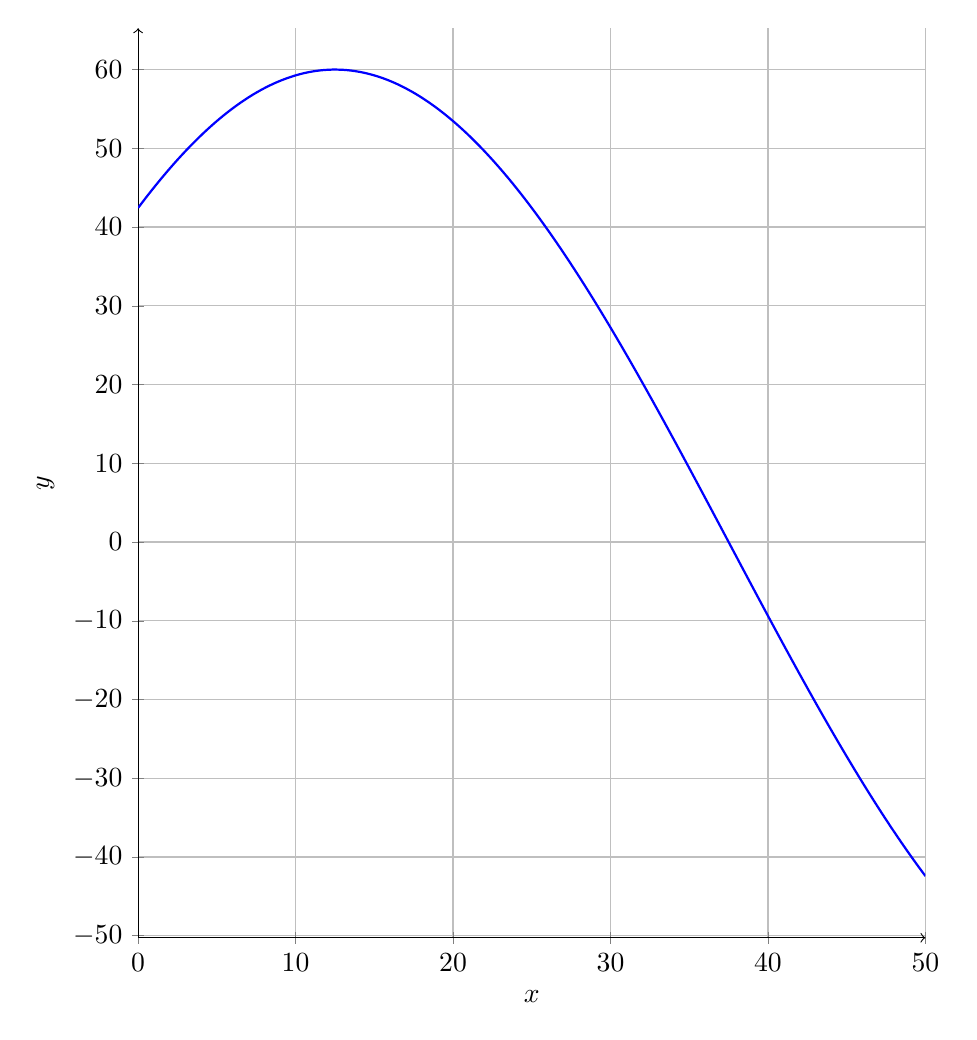
\begin{tikzpicture}
	\begin{axis}[
		axis x line=bottom,
		axis y line=left,
		xlabel={$x$}, ylabel={$y$},
		xmin=0, xmax=50,              % x-axis 0 to 50
		ymin=-45, ymax=60,            % y-axis -60 to 60
		xtick={0,10,...,50},          % x ticks every 10
		ytick={-60,-50,...,60},       % y ticks every 10
		grid=both,
		width=12cm, height=6cm,
		samples=200,
		domain=0:50,
		axis line style={->},         % arrows at ends
		% scale y visually double the x
		x=0.2cm,                      % compress x
		y=0.1cm,                      % stretch y
		enlarge y limits=0.05,
	]
		% scaled sine function to fit -60..60
		\addplot[blue, thick] {60*sin(deg((pi/50)*x + pi/4))};
	\end{axis}
	\end{tikzpicture}
\end{image}


% ik zou durven opteren voor onderstaande figuur, dan heb je bewegend voorwerp naast de grafiek staan, handig voor volgende situaties van snelheid en versnelling.

\begin{image}
\includegraphics[width=0.8\textwidth]{positiemetgrafiek}

\end{image}
\captionof{figure}{Links het verplaatsend voorwerp met begin- en eindpositie. Rechts de grafiek van \(x(t)\).}


De \textbf{verplaatsing} tussen $t_1$ en $t_2$ is verschil in positie tussen de twee tijdstippen $t_1$ en $t_2$, genoteerd met een $\Delta$\(\vec{r}\) (Delta, een Griekse hoofdletter D  van het Engelse 'displacement' of het Franse 'déplacement').

\begin{definition}
De \textbf{verplaatsing} \(\Delta \vec{r}\) is het verschil tussen twee posities:
\[
\Delta \vec{r} = \vec{r}_2 - \vec{r}_1
\]

\tikzset{>={latex[scale=1.2]}}

\begin{image}
	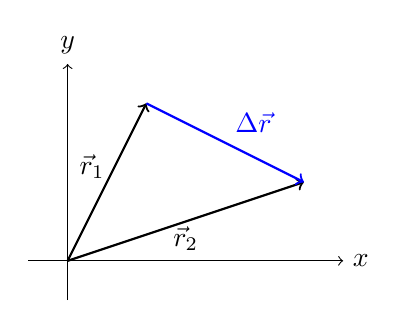
\begin{tikzpicture}
		
		\draw[->] (-0.5,0) -- (3.5,0) node[right] {$x$};
		\draw[->] (0,-0.5) -- (0,2.5) node[above] {$y$};
		
		\coordinate (X) at (1,2);
		\coordinate (Y) at (3,1);
		
		% \fill (X) circle (2pt) node[above] {};
		% \fill (Y) circle (2pt) node[above right] {};
		
		\draw[->, thick] (0,0) -- (X) node[pos= 0.6, left] {$\vec{r}_1$};
		\draw[->, thick] (0,0) -- (Y) node[midway, below, yshift=2pt] {$\vec{r}_2$};
		\draw[->, thick, blue] (X) -- (Y) node[midway, above right] { $\Delta \vec{r}$};
		
	\end{tikzpicture}
\end{image}
\end{definition}
% TODO: opmerking toevoegen dat de natatie $\Delta$ *erg* slecht is, omdat ze de indices 1 en 2 niet bevat!

Voor ééndimensionale bewegingen is de verplaatsing eenvoudig scalair te berekenen met: $\Delta x$ = $x_{eind}-x_{begin}$ .
In figuur 1 is de verplaatsing van de auto tussen de tijdstippen $t_0$ en $t_1$ gelijk aan $\Delta x = x_1-x_0=50\rm\,m-30\rm\,m=20\rm\,m$ en is de verplaatsing tussen de tijdstippen $t_2$ en $t_4$ gelijk aan $\Delta x=x_4-x_2=-40\rm\,m-40\rm\,m=-80\rm\,m$. Deze laatste verplaatsing is negatief, wat aangeeft dat de auto netto naar achteren is bewogen -- tegengesteld aan de zin van de gekozen as.

%%%\newline
Let op, de verplaatsing hoeft niet noodzakelijk gelijk te zijn aan de \emph{afgelegde weg} tussen de twee bijbehorende tijdstippen. Als je een rondje hebt gelopen op de atletiekpiste en terug aan start staat is je (netto) verplaatsing nul, maar heb je wel degelijk afstand afgelegd.

Samengevat:

\begin{image}
\includegraphics[width=0.8\textwidth]{positieverplaatsing1D}

\end{image}

Voor tweedimensionale bewegingen worden de begrippen positie, verplaatsing en afgelegde weg complexer.

\begin{image}
\includegraphics[width=0.8\textwidth]{positie2D}

\end{image}

\begin{image}
\includegraphics[width=0.8\textwidth]{verplaatsing2D}

\end{image}

	
\end{document}


